\documentclass{article}
\usepackage[T1]{fontenc}
\usepackage{lmodern}
\usepackage{graphicx}
\usepackage{amsmath,amssymb}
\usepackage[a4paper,margin=2cm]{geometry}
\usepackage[absolute,overlay]{textpos}
\setlength{\TPHorizModule}{1mm}
\setlength{\TPVertModule}{1mm}
\usepackage[indonesian]{babel}
\usepackage{hyperref}
\setlength{\emergencystretch}{2em}
% unit: Halaman 27

\begin{document}

% === Halaman 27 (llm) ===

\section*{Public Key Cryptography using RSA algorithm}
by: Syed Umar Anis

Purpose of the page is to demonstrate how RSA algorithm works - generates keys, encrypts message and decrypts it.

See the related blog post for more explanation.

\vspace{10mm}

\subsection*{Step \# 1: Generate Private and Public keys}

Enter two prime numbers below (P, Q), then press calculate:

\begin{itemize}
    \item P: 17
    \item Q: 29
\end{itemize}

\vspace{56.43mm}

Some prime numbers: 11, 13, 17, 19, 23, 29, 191, 193, 197, 199, etc.

\vspace{5mm}

% deskripsi: Tabel kalkulasi RSA yang menunjukkan variabel N (modulus) dan L (length) beserta nilai, nama, formula, dan deskripsinya.
% bbox normalisasi: [0.0400, 0.7800, 0.9500, 0.9700]
\begin{textblock*}{191.10mm}(8.40mm,231.66mm)
\noindent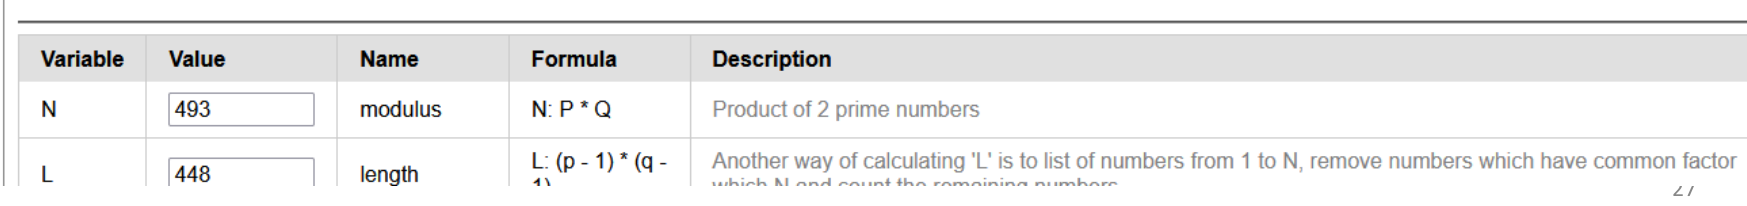
\includegraphics[width=191.10mm,height=56.43mm]{../../images/llm/page_027_img_01.png}%
\end{textblock*}

\end{document}
